\chapter{Løsningsimplementering}
Arbeidet i denne fasen går ut på å utrede en tiltaksplan og lage et forslag til hvordan dette skal implementeres. I den foregående fasen ble løsningene til rotårsakene identifisert. Vi kom fram til fire tiltak som vil fjerne rotårsaken. Tiltakene kan deles inn i to deler, en for eksterne og en for interne. Den eksterne løsningen går på det tekniske og den interne går på IT-reglementet. 

Den eksterne løsningen er å øke ressursene til seksjonen for digital sikkerhet gjennom å ansatte flere eller å bruke bachelorstudenter til å utføre blokkering av DNS-forespørsler tilknyttet kryptoutvinning.

Den interne løsningen er å tydeliggjøre at det å drive kryptoutvinning på NTNU ikke er lovlig og gjennomføre enn informasjonskampanje rundt dette.

\section{Kraftfeltsanalyse}
Kraftfeltsanalyse er et verktøy som analyserer hva som hjelper og hva som hindrer implementering av tiltaket.  

\subsection{Ønsket utbytte}
Ønsket utbytte fra kraftfeltsanalyse er å få vite hva som er for og hva som er imot implementering av tiltakene. Dette verktøyet gir en plan over hvilke tiltak som er lettest å gjennomføre. 

\subsection{Gjennomføring}
Kraftfeltsanalysen ble gjort ved at vi tok tiltakene fra problemelimineringen og hadde en idémyldring for å se hva som talte for tiltakene og hva som var imot. 

\subsection{Resultat}
 Under har vi de fire kraftfeltsanalysene
 
 Informasjonskampanjen og endringen i IT-reglementet bør gjøre i kombinasjon med hverandre. Der IT-reglementet får klartgjort at selv om kryptoutvinning ikke ulovlig i henhold til norsk lov, er det imot NTNU sitt IT-reglement så langt det ikke er søkt om. Når endringen er gjort, gjennomføres informasjonskampanjen.   
 Under, i tabell \ref{fig:kampanje} og \ref{fig:IT-reglement}, viser resultatene fra kraftfeltsanalyse på informasjonskampanje og endring i IT-reglementet.
 \begin{figure}[H]
    \hspace{2.2cm}
    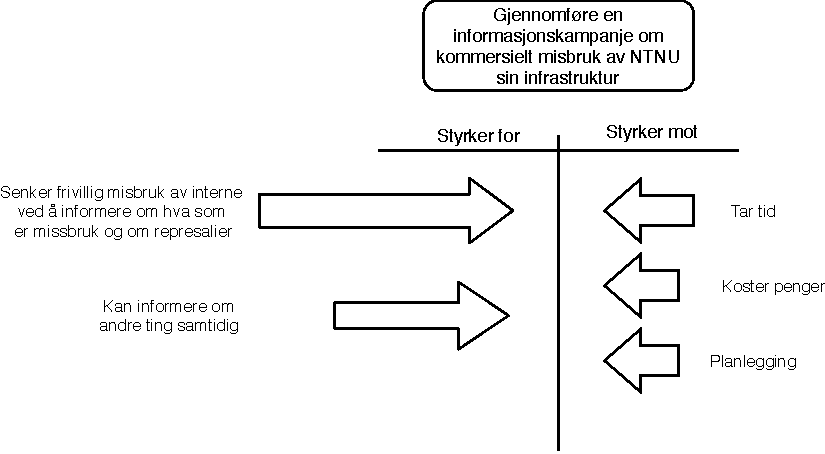
\includegraphics[scale=0.6]{case_3/bilder/Force-field1.pdf}
    \caption[Informasjonskampanje]{Oversikt over informasjonskampanjen }
    \label{fig:kampanje}
\end{figure}

 
 \begin{figure}[H]
    \hspace{2.6cm}
    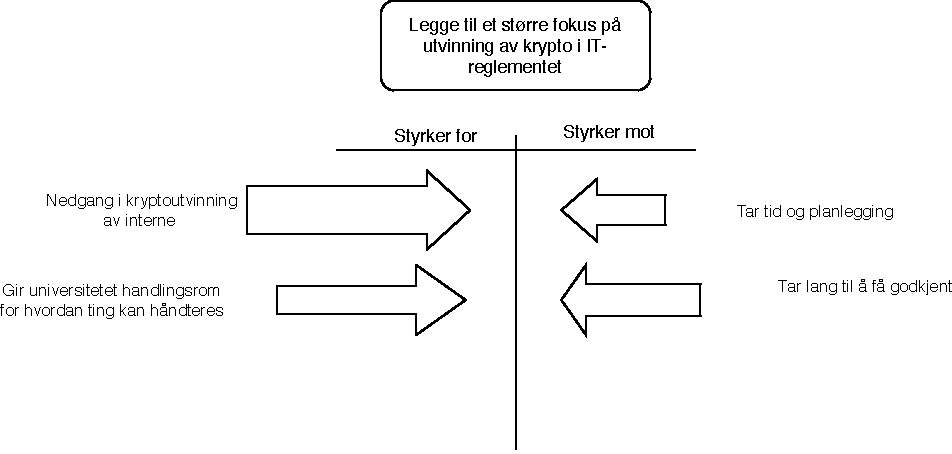
\includegraphics[scale=0.6]{case_3/bilder/Force-field2.pdf}
    \caption[Endre IT-reglementet]{Endring i IT-reglementet}
    \label{fig:IT-reglement}
\end{figure}

Fra dataanalysen kom fram til at selv om det finnes tekniske løsninger, har ikke SOCen hatt mulighet til å implementere DNS blokkering på bakgrunn av mangel på ressurser. Figur \ref{fig:Blokkering} og \ref{fig:Oke-antall} viser hva som skal til for å blokkere DNS og hva som må til for å øke ressursene til SOCen.    
 \begin{figure}[H]
    \centering
    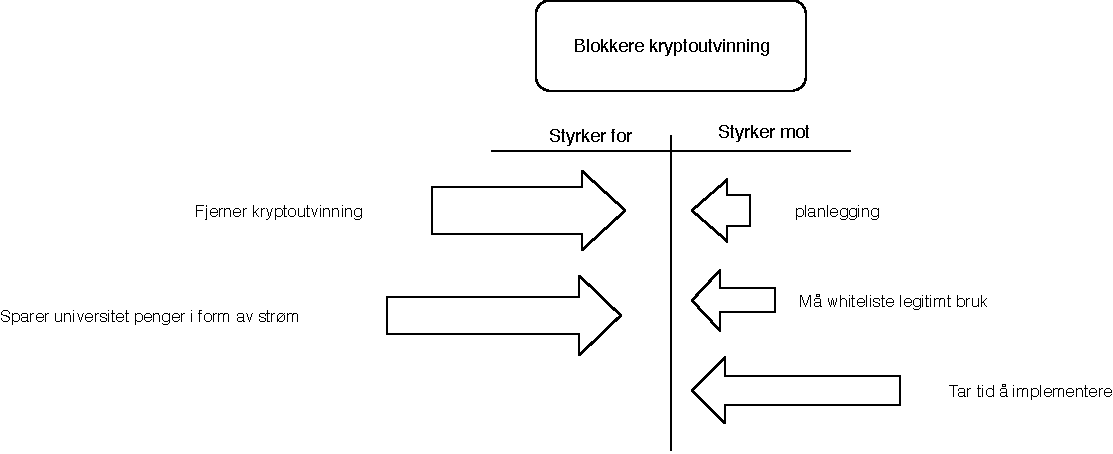
\includegraphics[scale=0.6]{case_3/bilder/Force-Field3.pdf}
    \caption[Blokkering]{Blokkering av DNS forespørsel}
    \label{fig:Blokkering}
\end{figure}

 \begin{figure}[H]
    \hspace{3.6cm}
    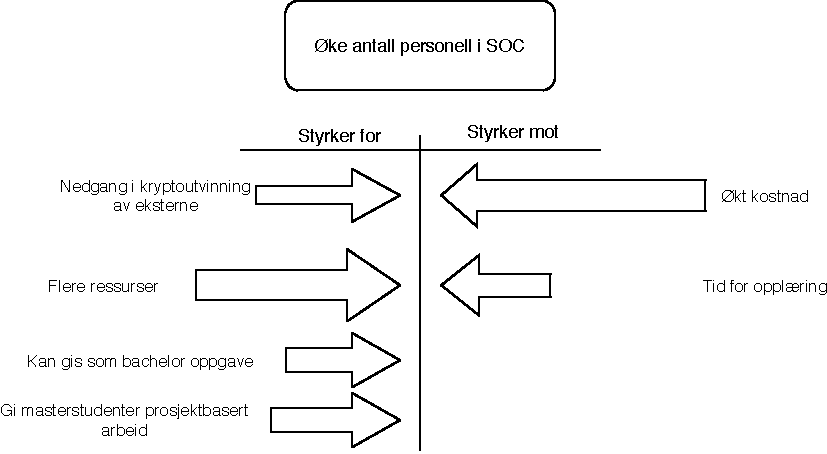
\includegraphics[scale=0.6]{case_3/bilder/Force-field4.pdf}
    \caption[Øke antall ansette i SOC]{Øke andel ansatte i SOC}
    \label{fig:Oke-antall}
\end{figure}

Figurene viser våres antakelser på hva som jobber for implementeringen og hva som jobber imot samt  estimater på styrken til antakelsene. 
\subsection{Konklusjon av verktøyet}
Verktøyet har potensiale til å fungere bra, der oversikten man får er bra så lenge datagrunnlaget er godt. Problemmet vårt var at vi jobbet med antakelser og ikke et datasett. Vi hadde ikke tid til å undersøke estimatene, så de har en høy usikkerhet.     